\section{Сравнение оценок}

\subsection{Общие определения}

\begin{definition}
    Функцией потерь называется любая борелевская неотрицательная функция $g(x, y)$, $x, y \in \R^n,\ g \colon \R^n \times \R^n \to \R$.
\end{definition}

\begin{note}
    Мне не очень нравится это определение на самом деле. В таком случае мы считаем функцией потерь $g(x, y) \equiv 1$, но не считаем функцией потерь $g(x, y) = \|x - y\|_2 - 1$, хотя вторая функция для потерь подходит лучше.
\end{note}

\begin{definition}
    Если $\theta^*(X)$ -- оценка параметра $\theta$, то функция $g(\theta^*(X), \theta)$, где $g$ -- функция потерь, называется величиной потерь.
\end{definition}

\begin{example}~
    \begin{enumerate}
        \item $g(x, y) = |x-y|,\ x, y \in \R$
        \item $g(x, y) = (x-y)^2,\ x, y \in \R$ -- квадратичная функция потерь
        \item $g(x, y) = \tbr{A(x-y), x-y} = (x-y)^T A^T (x-y) = (x-y)^T A (x-y)$, где $A$ -- неотрицательно определённая (симметричная) матрица, $x, y \in \R^n$
    \end{enumerate}
\end{example}

\begin{definition}
    Если задана функция потерь $g$, то функцией риска оценки $\theta^*(X)$ называется функция $R(\theta^*, \theta) = \E_\theta g(\theta^*(X), \theta)$.
\end{definition}

\begin{note}
    Для того, чтобы можно было брать математическое ожидание, в определении функции потерь и требовали борелевость.
\end{note}

\begin{note}
    Если оценки $\theta^*(X)$ и $\hat{\theta}(X)$ совпадают $P_\theta$-почти наверное для всех $\theta$, например, отличаются в одной точке в случае семейства абсолютно непрерывных распределений, то они имеют одинаковую функцию риска. Такие оценки различать не будем, будем считать одной и той же оценкой в рамках подходов, которые используют функцию риска.
\end{note}

\subsection{Различные подходы к сравнению оценок}

\subsubsection{Равномерный подход}

\begin{definition}
    Оценка $\hat{\theta}(X)$ лучше оценки $\theta^*(X)$ в равномерном подходе, если у неё меньше риск $R(\hat{\theta}, \theta) \le R(\theta^*, \theta) \ \forall \theta \in \Theta$, и для некоторого $\theta$ неравенство строгое.
\end{definition}

\begin{definition}
    Оценка $\hat{\theta}$ называется наилучшей в равномерном подходе в классе оценок $K$, если она лучше любой другой оценки $\theta^* \in K$. Если оценка одна в своём классе, то она, разумеется, наилучшая.
\end{definition}

\begin{note}
    Наилучшая оценка существует не всегда. Например, рассмотрим квадратичную функцию потерь $g(x, y) = (x-y)^2$ и $K = \{\text{всевозможные оценки}\}$. Рассмотрим тождественные оценки $\hat{\theta_0}(X) \equiv \theta_0$, $\theta_0 \in \Theta$, они удовлетворяют соотношению $R(\hat{\theta_0}, \theta_0) \equiv 0$. Если $\theta^*$ -- наилучшая оценка, то она при любом $\theta \in \Theta$ лучше тождественной оценки, в частности, имеет нулевой риск $R(\theta^*, \theta) \equiv 0$. Это означает, что её величина потерь, в силу неотрицательности функции потерь, почти наверное равна нулю при каждом $\theta$. В общем случае так хорошо оценивать мы не умеем.

    Тем не менее, такая хорошая оценка может существовать в вырожденных случаях. Например, рассмотрим семейство распределений $\set{U\sbr{\theta, \theta+\frac{1}{2}},\ \theta \in \N}$. Тогда следующая оценка $\theta^*(x) = [x],\ x \in \R,\ [x]$ -- целая часть, однозначно определяет параметр $\theta$, поэтому имеет нулевую величину потерь в случае адекватной функции потерь.
\end{note}

\begin{note}
    Точно так же можем сравнивать в равномерном подходе оценки $\tau(\theta)$.
\end{note}

\begin{note}
    Если $g$ -- квадратичная функция потерь, $K$ -- класс несмещённых оценок для некоторой $\tau(\theta)$, то задача поиска наилучшей оценки, то есть оценки с наименьшим риском, сводится к поиску оценки с наименьшей дисперсией.
\end{note}

\subsubsection{Минимаксный подход}

\begin{note}
    Идея в том, что смотрим на самые <<страшные>> потери и пытаемся их сделать как можно меньше.
\end{note}

\begin{definition}
    Оценка $\theta^*$ называется наилучшей в минимаксном подходе в классе оценок $K$, если она имеет наименьшую функцию риска, то есть
    \[
        \sup_{\theta \in \Theta} R(\theta^*, \theta) = \inf_{\hat{\theta} \in K} \sup_{\theta \in \Theta} R(\hat{\theta}, \theta)
    \]
\end{definition}

\begin{note}
    Минимаксный подход плох, если одна оценка сильно лучше другой для большинства $\theta$, но немного хуже на небольшом участке, на котором и получаем супремум. На картинке ниже хочется сказать, что оценка, написанная ниже, лучше с точки зрения площади под графиком. Примерно эту идею и формализует байесовский подход.

    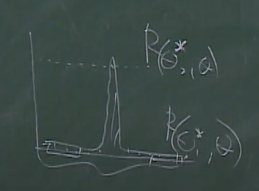
\includegraphics{images/picture1.png}
\end{note}

\subsubsection{Байесовский подход}

Предположим, что на $\Theta$ задано некоторое (априорное) распределение вероятности $Q$, и $\theta$ выбирается случайно в соответствии с распределением $Q$.

Идея заключается в том, что уже имеем некоторые предположения о том, какие $\theta$ более вероятны.

Обозначим $R(\hat{\theta}) = \int_\Theta R(\hat{\theta}, \theta) Q(d \theta)$, где $\hat{\theta}$ -- оценка, $R(\hat{\theta}, \theta)$ -- её функция риска.

\begin{definition}
    Оценка $\theta^*$ называется наилучшей в байесовском подходе в классе оценок $K$, если $R(\theta^*) = \inf_{\hat{\theta} \in K} R(\hat{\theta})$.
\end{definition}

\begin{example}
    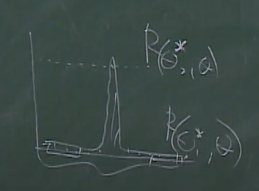
\includegraphics{images/picture1.png}

    На этой картинке оценка, написанная выше, лучше в минимаксном подходе, оценка, написанная ниже, лучше в байесовском подходе с априорным распределением $U[0, 1]$, где $[0, 1]$ -- отрезок на рисунке, в равномерном подходе эти оценки не сравнимы.
\end{example}

\subsubsection{Асимптотический подход}

\begin{definition}
    Пусть $\hat{\theta_1}$ и $\hat{\theta_2}$ -- две асимптотически нормальные оценки параметра $\theta$ с асимптотическими дисперсиями $\sigma_1^2(\theta)$ и $\sigma_2^2(\theta)$. $\hat{\theta_1}$ лучше $\hat{\theta_2}$ в асимптотическом подходе, если
    \[
        \sigma_1^2(\theta) \le \sigma_2^2(\theta) \ \ \forall \theta \in \Theta
    \]
\end{definition}

\begin{example}
    Пусть $X_1, \dots, X_n$ -- выборка из $N(\theta, 1)$. Сравним в асимптотическом подходе оценки среднее $\overline{X}$ и выборочную медиану $\hat{\mu}$.

    В силу ЦПТ:
    \[
        \sqrt{n}(\overline{X} - \theta) \xrightarrow{d} N(0, 1)
    \]
    
    В силу теоремы о выборочной медиане:
    \[
        \sqrt{n}(\hat{\mu} - \theta) \xrightarrow{d} N\ps{0, \frac{1}{4 f^2(\theta)}} = N\ps{0, \frac{\pi}{2}}
    \]
    
    Здесь использовали, что плотность нормального распределения $N(\theta, 1)$:
     \[
        f(x) = \frac{1}{\sqrt{2 \pi}} e^{-\frac{(x-\theta)^2}{2}}
     \]

     То есть в асимптотическом подходе среднее лучше, но медиана на практике тоже полезна, так как более устойчива к выбросам.
\end{example}

\begin{definition}
    Оценка $\hat{\theta}$ называется наилучшей в асимптотическом подходе в классе $K$, содержащем асимптотически нормальные оценки, если она лучше любой другой оценки $\theta^* \in K$.
\end{definition}

\subsection{Понятие плотности дискретного распределения}

Не очень к теме, не очень интересно, было на теории вероятностей и можно посмотреть в конспекте лекций Савёлова за 2023 год.

\subsection{Эффективные оценки}

\begin{definition}
    Среднеквадратичный подход к сравнению оценок -- это равномерный подход с квадратичной функцией потерь.
\end{definition}

\begin{proposition}
    Пусть $K$ -- класс несмещённых оценок для $\tau(\theta)$. Если $T_1, T_2 \in K$, такие, что
    \[
        \E_\theta (T_1 - \tau(\theta))^2 = \E_\theta (T_2 - \tau(\theta))^2 = \inf_{T \in K} E(T - \tau(\theta))^2 \ \ \forall \theta \in \Theta
    \]
    то $T_1 = T_2 \ P_\theta\text{-п.н.} \ \forall \theta \in \Theta$. То есть наилучшая оценка в среднеквадратичном подходе единственна с точностью до множеств нулевой вероятности.
\end{proposition}

\begin{note}
    Кажется, что нужно ещё потребовать $\E_\theta (T_1 - \tau(\theta))^2 < \infty \ \ \forall \theta \in \Theta$, иначе ни это доказательство, ни доказательство из конспекта лекций Савёлова 2023 года не проходят.
\end{note}

\begin{proof}
    Рассмотрим $\frac{T_1+T_2}{2}$. Так как приняли наиболее общее определение оценки, в котором не требуем, что её множество значений вложено в $\tau(\theta)$, то $\frac{T_1+T_2}{2}$ тоже является оценкой параметра $\tau(\theta)$, причём несмещённой, то есть $\frac{T_1+T_2}{2} \in K$. Тогда получим, что
    \begin{multline*}
        E_\theta \ps{\frac{T_1+T_2}{2} - \tau(\theta)}^2 = E_\theta \ps{\frac{T_1-\tau(\theta)}{2} + \frac{T_2-\tau(\theta)}{2}}^2 =
        \\
        = \frac{1}{4} \E_\theta (T_1 - \tau(\theta))^2 + \frac{1}{4} \E_\theta (T_2 - \tau(\theta))^2 + \frac{1}{2} \E_\theta (T_1 - \tau(\theta)) (T_2 - \tau(\theta))
    \end{multline*}

    В силу неравенства Коши-Буняковского-Шварца:
    \begin{multline*}
        \E_\theta (T_1 - \tau(\theta)) (T_2 - \tau(\theta)) \le |\E_\theta (T_1 - \tau(\theta)) (T_2 - \tau(\theta))| \le
        \\
        \le \sqrt{\E_\theta (T_1 - \tau(\theta))^2 \E_\theta (T_2 - \tau(\theta))^2} = \E_\theta (T_1 - \tau(\theta))^2
    \end{multline*}

    Таким образом, с учётом условия, получаем:
    \[
        \E_\theta \ps{\frac{T_1+T_2}{2} - \tau(\theta)}^2 \le \ps{\frac{1}{4}+\frac{1}{4}+\frac{1}{2}} \E_\theta (T_1 - \tau(\theta))^2 \le \E_\theta \ps{\frac{T_1+T_2}{2} - \tau(\theta)}^2
    \]

    Тогда во всех неравенствах достигается равенство, в частности:
    \begin{align*}
        & \E_\theta (T_1 - \tau(\theta)) (T_2 - \tau(\theta)) \ge 0
        \\
        & |\E_\theta (T_1 - \tau(\theta)) (T_2 - \tau(\theta))| = \sqrt{\E_\theta (T_1 - \tau(\theta))^2 \E_\theta (T_2 - \tau(\theta))^2}
    \end{align*}

    Напомним, что равенство в КБШ достигается тогда и только тогда, когда векторы линейно зависимы, то есть:
    \[
        a(\theta) (T_1 - \tau(\theta)) = b(\theta) (T_2 - \tau(\theta)) \ P_\theta\text{-п.н.}
    \]

    Попробуем извлечь отсюда выводы про $a(\theta)$ и $b(\theta)$:
    \begin{align*}
        & \E_\theta (T_1 - \tau(\theta)) (T_2 - \tau(\theta)) \ge 0
        \\
        & a(\theta)^2 \E_\theta (T_1 - \tau(\theta))^2 = b(\theta)^2 \E_\theta (T_2 - \tau(\theta))^2 = b(\theta)^2 \E_\theta (T_1 - \tau(\theta))^2
        \\
        & a(\theta) b(\theta) \E_\theta (T_1 - \tau(\theta)) (T_2 - \tau(\theta)) = \E_\theta (a(\theta) (T_1 - \tau(\theta)))^2 \ge 0
    \end{align*}

    Если $\E_\theta (T_1 - \tau(\theta))^2 = \E_\theta (T_2 - \tau(\theta))^2 = 0$, то $T_1 = T_2 = \tau(\theta) \ P_\theta\text{-п.н.}$, и всё доказано, далее считаем, что $\E_\theta (T_1 - \tau(\theta))^2 > 0$. Тогда $a(\theta)^2 = b(\theta)^2$, причём, так как эти коэффициенты появились из линейной зависимости, то они не оба ненулевые, следовательно, оба ненулевые. Тогда $a(\theta) b(\theta) \E_\theta (T_1 - \tau(\theta)) (T_2 - \tau(\theta)) = a(\theta)^2 \E_\theta (T_1 - \tau(\theta)) (T_2 - \tau(\theta)) > 0$, с учётом первого из неравенств выше $a(\theta) b(\theta) > 0$. Тогда
    \[
        a(\theta)^2 = b(\theta)^2 \text{ и } a(\theta) b(\theta) > 0 \Ra a(\theta) = b(\theta) \neq 0
    \]

    Отсюда вытекает:
    \[
        T_1 - \tau(\theta) = T_2 - \tau(\theta) \ P_\theta\text{-п.н.} \Ra T_1 = T_2 \ P_\theta\text{-п.н.}
    \]
\end{proof}

\begin{definition}
    Семейство распределений $\{P_\theta,\ \theta \in \Theta\}$ называется доминируемым относительно меры $\mu$, если $\forall \theta \in \Theta \ P_\theta$ имеет плотность по одной и той же мере $\mu$. 
\end{definition}

\begin{note}
    Далее рассматриваем $\{P_\theta,\ \theta \in \Theta\}$ -- доминируемое семейство распределений относительно меры $\mu$, работаем в одномерном случае, то есть $\Theta \subset \R$, дана $X$ -- выборка из неизвестного распределения $P_\theta$, $p_\theta(X)$ есть функция правдоподобия.
\end{note}

\begin{definition}
    Случайная величина $U_\theta(X) = \frac{\partial}{\partial \theta} \ln p_\theta(X)$ называется вкладом выборки $X$, функция $I_X(\theta) = \E_\theta U_\theta^2(X)$ называется количеством информации о параметре $\theta$, содержащейся в $X$ (информацией Фишера).
\end{definition}

\begin{note}
    Информация Фишера $I_X(\theta)$ зависит от $X$ только через размер выборки. Если $X$ -- выборка размера 1, то информация Фишера обозначается как $i(\theta)$.
\end{note}

\begin{note}
    Почему такая терминология?
    \[
        U_\theta(X) = \frac{\partial}{\partial \theta} \ln p_\theta(X) = \sum_{i=1}^n \frac{1}{p_\theta(X_i)} \frac{\partial}{\partial \theta} p_\theta(X_i)
    \]
    Для каждого $i$ слагаемое является относительной скоростью изменения плотности по $\theta$, чем в среднем больше квадрат суммарной скорости, тем проще отличить $\theta_1$ и $\theta_2$.

    Конкретные детали определения зависят от хороших свойств, которые скоро сформулируем. Но прежде сформулируем некоторые требования, в рамках которых со всем этим будет осмыслено работать.
\end{note}

\begin{definition}
    Будем считать, что выполнены условия регулярности:
    \begin{itemize}
        \item[(R1)] $\Theta \subset \R$, $\Theta$ -- открытый интервал, возможно, бесконечный.

        \item[(R2)] Множество $A = \{x \in \cX : p_\theta(x) > 0\}$ не зависит от $\theta$, $A$ называется носителем. Здесь $x$ одномерный, то есть соответствует выборке размера 1.

        \item[(R3)] Для любой статистики $S(X)$ с условием $\E S^2(X) < \infty$ выполнено равенство, в частности, его левая и правая части существуют:
        \[
            \frac{\partial}{\partial \theta} \E_\theta S(X) = \E_\theta S(X) U_\theta(X)
        \]

        \item[(R4)] $0 < I_X(\theta) < \infty \ \ \forall \theta \in \Theta$
    \end{itemize}
\end{definition}

\begin{note}
    Теперь поймём смысл того, что здесь написано.

    \begin{itemize}
        \item[(R1)] Открытость нам нужна для того, чтобы дифференцировать, интервал, то есть связность, требуем для того, чтобы, например, из тождественно нулевой производной следовала постоянность функции.

        \item[(R2)] Во-первых, по сути, $A$ -- это разрешённое множество значений для выборки $X$, то есть запрещаем ситуацию, когда какому-то из распределений нельзя принимать некоторые значения, допустимые для других распределений. Во-вторых, это будет нужно для того, чтобы аккуратно расписать интеграл в (R3).

        \item[(R3)] Будет ниже.

        \item[(R4)] Так как по определению информация Фишера неотрицательна, такое требование разумно и нужно, чтобы на информацию Фишера можно было делить.
    \end{itemize}
\end{note}

\begin{reminder} (Теорема о дифференцируемости собственного интеграла по параметру)
	Пусть даны $f \colon E \times (c; d) \to \R$, где $E \subseteq \R^m$ --- измеримое множество. Если выполнены следующие условия :
	\begin{enumerate}
		\item Для любого $\alpha \in (c; d)$ функция $f(x, \alpha)$ суммируема на $E$
		
		\item Для любого $\alpha \in (c; d)$ почти всюду на $E$ верно неравенство $\md{\pd{f}{\alpha}(x, \alpha)} \le \phi(x)$, где $\phi \in L_1(E)$
	\end{enumerate}
	Тогда взятие производной по параметру коммутирует с интегралом по $E$ (ну или можно сказать, что оператор производной вносится под знак интеграла):
	\[
		\forall \alpha \in (c; d)\ \ \pd{}{\alpha} \ps{\int_E f(x, \alpha)d\mu(x)} = \int_E \pd{}{\alpha}f(x, \alpha)d\mu(x)
	\]
\end{reminder}

\begin{note}~
    \begin{itemize}
        \item[(R3)] Перепишем требование в немного другом виде:
        \begin{multline*}
            \frac{\partial}{\partial \theta} \E_\theta S(X) = \frac{\partial}{\partial \theta} \int_{A^n} S(X) p_\theta(X) \mu(dX) \overset{?}{=} \int_{A^n} \frac{\partial}{\partial \theta} [S(X) p_\theta(X)] \mu(dX) =
            \\
            = \int_{A^n} S(X) \frac{\partial}{\partial \theta} p_\theta(X) \mu(dX) = \int_{A^n} S(X) U_\theta(X) p_\theta(X) \mu(dX) = E_\theta S(X) U_\theta(X)
        \end{multline*}

        То есть вопрос в том, можем ли внести производную под интеграл. Так как $A^n$ измеримо, а $\Theta$ -- интервал, по теореме выше достаточно проверить суммируемость подинтегральной функции и то, что её можно продифференцировать, а результат мажорировать суммируемой функцией.

        Теперь откуда взялось $S^2(X) < \infty$? Как я понимаю, оно унаследовалось из книги Боровкова по математической статистике, а там использовалось для доказательства корректности внесения производной под интеграл вместе с некоторыми дополнительными предположениями.
    \end{itemize}
\end{note}

\begin{proposition}~
    \begin{enumerate}
        \item $\E_\theta U_\theta(X) = 0$
        \item $I_X(\theta) = n i(\theta)$
    \end{enumerate}
\end{proposition}

\begin{proof}~
    \begin{enumerate}
        \item Применим условие регулярности (R3) для статистики $S(X) \equiv 1$:
        \[
            \E_\theta U_\theta(X) = \E_\theta S(X) U_\theta(X) = \frac{\partial}{\partial \theta} \E_\theta S(X) = \frac{\partial}{\partial \theta} 1 = 0 
        \]

        \item Распишем по определению, воспользуемся независимостью элементов выборки:
        \begin{multline*}
            I_X(\theta) = \E_\theta U_\theta^2(X) = \E_\theta \ps{\frac{\partial}{\partial \theta} \ln p_\theta(X)}^2 = \E_\theta \ps{\sum_{i=1}^n \frac{\partial}{\partial \theta} \ln p_\theta(X_i)}^2 =
            \\
            = \sum_{i=1}^n \E_\theta \ps{\frac{\partial}{\partial \theta} \ln p_\theta(X_i)}^2 + \sum_{i,j=1}^n \E_\theta \ps{\frac{\partial}{\partial \theta} \ln p_\theta(X_i)} \ps{\frac{\partial}{\partial \theta} \ln p_\theta(X_j)} =
            \\
            = \sum_{i=1}^n \E_\theta \ps{\frac{\partial}{\partial \theta} \ln p_\theta(X_i)}^2 + \sum_{i,j=1}^n \E_\theta \ps{\frac{\partial}{\partial \theta} \ln p_\theta(X_i)} \E_\theta \ps{\frac{\partial}{\partial \theta} \ln p_\theta(X_j)} =
            \\
            = \sum_{i=1}^n i(\theta) + \sum_{i,j=1}^n (\E_\theta U_\theta(X_1))^2 = n i(\theta)
        \end{multline*}
    \end{enumerate}
\end{proof}

\begin{theorem} (Неравенство Рао-Крамера)
    Пусть выполнены условия регулярности и $\hat{\theta}(X)$ -- несмещённая оценка $\tau(\theta)$ с условием $\E_\theta (\hat{\theta}(X))^2 < \infty \ \forall \theta \in \Theta$. Тогда
    \[
        D_\theta \hat{\theta}(X) \ge \frac{(\tau'(\theta))^2}{I_X(\theta)} = \frac{(\tau'(\theta))^2}{n i(\theta)}
    \]
\end{theorem}

\begin{note}
    Смысл теоремы: в среднеквадратичном подходе для несмещённых оценок ищется оценка с наименьшей дисперсией. Здесь получаем оценку снизу на дисперсию.
\end{note}

\begin{proof}
    Применим условие регулярности (R3) для статистики $S(X) = \hat{\theta}(X)$:
    \[
        \E_\theta \hat{\theta}(X) U_\theta(X) = \frac{\partial}{\partial \theta} \E_\theta \hat{\theta}(X) = \frac{\partial}{\partial \theta} \tau{\theta} = \tau'(\theta)
    \]

    Перепишем в немного другом виде:
    \[
        \tau'(\theta) = \E_\theta \hat{\theta}(X) U_\theta(X) = \E_\theta \hat{\theta}(X) U_\theta(X) - \tau(\theta) \E U_\theta(X) = \E_\theta [\hat{\theta}(X) - \tau(\theta)]  U_\theta(X)
    \]

    Воспользуемся неравенством Коши-Буняковского-Шварца:
    \[
        | \tau'(\theta) |^2 = | \E_\theta [\hat{\theta}(X) - \tau(\theta)] U_\theta(X) |^2 \le \E_\theta [\hat{\theta}(X) - \tau(\theta)]^2 \E_\theta (U_\theta(X))^2 = \E_\theta [\hat{\theta}(X) - \tau(\theta)]^2 I_X(\theta)
    \]

    В силу несмещённости оценки $\E_\theta (\hat{\theta}(X) - \tau(\theta))^2 = D_\theta \hat{\theta}(X)$, в силу (R4) $I_X(\theta) > 0$:
    \[
        \frac{|\tau'(\theta)|^2}{I_X(\theta)} \le D_\theta \hat{\theta}(X)
    \]
\end{proof}

\begin{corollary}
    Пусть выполнены условия регулярности и $\hat{\theta}(X)$ -- несмещённая оценка $\theta$ с условием $\E_\theta (\hat{\theta}(X))^2 < \infty \ \forall \theta \in \Theta$. Тогда
    \[
        D_\theta \hat{\theta}(X) \ge \frac{1}{I_X(\theta)} = \frac{1}{n i(\theta)}
    \]
\end{corollary}

\begin{definition}
    Если в неравенстве Рао-Крамера для несмещённой оценки $\hat{\theta}(X)$ достигается равенство (отсюда следует конечность второго момента), то $\hat{\theta(X)}$ называется эффективной оценкой $\tau(\theta)$.
\end{definition}

\begin{theorem} (Критерий эффективности)
    В условиях регулярности следующие утверждения эквивалентны:
    \begin{enumerate}
        \item $\hat{\theta(X)}$ -- эффективная оценка $\tau(\theta)$
        \item $\hat{\theta}(X)$ -- линейная функция от $U_\theta(X)$ вида:
        \[
            \hat{\theta}(X) - \tau(\theta) = c(\theta) U_\theta(X) \ P_\theta \text{-п.н.} \text{ -- для некоторой } c(\theta)
        \]
    \end{enumerate}

    При этом последнее равенство выполнено тогда и только тогда, когда $c(\theta) = \frac{\tau'(\theta)}{I_X(\theta)}$.    
\end{theorem}

\begin{proof}
    Идея доказательства состоит в том, что неравенство Рао-Крамера вытащили из неравенства Коши-Буняковского-Шварца, значит, надо посмотреть, когда в последнем достигается равенство.

    Сначала проверим, что для оценок из обоих пунктов выполнены условия теоремы о неравенстве Рао-Крамера. В первом случае это очевидно. Во втором случае: распишем математическое ожидание $\E_\theta \hat{\theta}(X) = c(\theta) \E_\theta U_\theta(X) + \tau(\theta) = \tau(\theta)$, отсюда получили несмещённость, и дисперсию $D_\theta \hat{\theta}(X) = c(\theta)^2 \E_\theta U_\theta^2(X) = c(\theta)^2 I_X(\theta) < \infty$, отсюда получили конечность второго момента.

    Теперь посмотрим, когда в неравенстве КБШ
    \[
        | \E_\theta [\hat{\theta}(X) - \tau(\theta)] U_\theta(X) |^2 \le \E_\theta [\hat{\theta}(X) - \tau(\theta)]^2 \E_\theta (U_\theta(X))^2
    \] достигается равенство. Тогда и только тогда, когда случайные величины линейно зависимы, то есть $a(\theta) [\hat{\theta}(X) - \tau(\theta)] = b(\theta) U_\theta(X) \ P_\theta \text{-п.н.}$. Если для некоторого $\theta$ $a(\theta) = 0$, то выполнено $0 = \E_\theta (b(\theta) U_\theta(X))^2 = b(\theta)^2 I_X(\theta)$, а из условий регулярности $I_X(\theta) > 0$, следовательно, $b(\theta) = 0$, что невозможно, так как $a(\theta)$ и $b(\theta)$ пришли из определения линейной зависимости. Тогда $a(\theta)$ не обращается в ноль, и можем переписать в виде $\hat{\theta}(X) - \tau(\theta) = c(\theta) U_\theta(X) \ P_\theta \text{-п.н.}$

    Таким образом, доказали эквивалентность, потому что если оценка эффективная, то в КБШ есть равенство, тогда оценка линейно зависит от вклада выборки. Если оценка линейно зависит от вклада выборки в виде из условия, то проходя через доказательство неравенства Рао-Крамера, получим, что там достигнется равенство.

    Осталось найти конкретный вид $c(\theta)$:
    \begin{align*}
        & \hat{\theta}(X) - \tau(\theta) = c(\theta) U_\theta(X) \ P_\theta \text{-п.н.}
        \\
        & (\hat{\theta}(X) - \tau(\theta)) U_\theta(X) = c(\theta) U_\theta^2(X) \ P_\theta \text{-п.н.}
        \\
        & \E (\hat{\theta}(X) - \tau(\theta)) U_\theta(X) = c(\theta) I_X(\theta)
    \end{align*}

    При доказательстве неравенства Рао-Крамера получили, что $\tau'(\theta) = \E_\theta [\hat{\theta}(X) - \tau(\theta)]  U_\theta(X)$, так что $\tau'(\theta) = c(\theta) I_X(\theta)$ и всё доказано.
\end{proof}

\begin{note}
    В доказательстве на лекции этого критерия, кажется, была бага, так как утверждалось, что в КБШ есть равенство тогда и только тогда, когда $\alpha(\theta) [\hat{\theta}(X) - \tau(\theta)] + \beta(\theta) U_\theta(X) + \gamma(\theta) = 0 \ P_\theta \text{-п.н.}$, но линейная зависимость в пространстве Лебега $L_2(\R)$ работает немного не так.
\end{note}

\begin{corollary}
    Если $\theta^*$ и $\hat{\theta}$ -- две эффективные оценки $\tau(\theta)$, то $\theta^* = \hat{\theta} \ P_\theta \text{-п.н.} \ \forall \theta \in \Theta$. Это следует не только из критерия эффективности, но и из утверждения про единственность наилучшей оценки среди несмещённых в среднеквадратичном подходе.
\end{corollary}

\begin{note}
    Эффективная оценка $\tau(\theta)$ -- наилучшая оценка $\tau(\theta)$ -- наилучшая оценка $\tau(\theta)$ в классе несмещёных $L_2$-оценок в равномерном подходе с квадратичной функцией потерь.

    Кажется, что $L_2$ здесь можно не требовать, так как эффективная оценка имеет конечную дисперсию, а оценки не из $L_2$ имеют бесконечную дисперсию.

    В обратную сторону неверно: наилучшая оценка $\tau(\theta)$ в классе несмещёных $L_2$-оценок в равномерном подходе с квадратичной функцией потерь не обязательно является эффективной.
\end{note}

\begin{note}
    На многомерный случай неравенство Рао-Крамера обобщается через неравенства через неотрицательную определённость матриц, но не будем на этом останавливаться.
\end{note}

\begin{note}
    Теперь результат о том, что существование эффективной оценки является редкостью, но сначала вспомогательная лемма.
\end{note}

\begin{lemma}
     Пусть $\{P_\theta,\ \theta \in \Theta\}$ -- доминируемое семейство распределений относительно меры $\mu$, множество $A = \{x \in \cX : p_\theta(x) > 0\}$ не зависит от $\theta$. Тогда $\forall B \in \B(\cX)$ эквивалентно:
     \begin{enumerate}
         \item $\exists \theta_0 \in \Theta \ \ P_{\theta_0}(B) = 1$
         \item $\forall \theta \in \Theta \ \ P_\theta(B) = 1$
     \end{enumerate}
\end{lemma}

\begin{proof}
    Понятно, что интересна только импликация $1 \Ra 2$. Пойдём от противного: предположим, что существует $\theta$, для которого $P_\theta(B) < 1$.

    Тогда получим:
    \begin{align*}
        & P_{\theta_0}(\cX \setminus B) = \int_{\cX \setminus B} p_{\theta_0}(x) \mu(dx) = 0
        \\
        & P_\theta(\cX \setminus B) = \int_{\cX \setminus B} p_\theta(x) \mu(dx) > 0
    \end{align*}

    Так как плотность неотрицательна, то множество $\{x \in \cX \setminus B : p_{\theta_0}(x) > 0\}$ имеет нулевую меру, множество $\{x \in \cX \setminus B : p_\theta(x) > 0\}$ имеет ненулевую меру. Противоречие с тем, что $A$ не зависит от $\theta$.
\end{proof}

\begin{theorem}
    Если в условиях регулярности есть эффективная оценка для $\tau(\theta) \not\equiv const$, то множество функций, для которых существует эффективная оценка, можно записать в виде $\{a \tau(\theta) + b\}$, $a, b \in \R$, $a, b = const$.
\end{theorem}

\begin{note}
    Случай $\tau(\theta) \equiv const$ в принципе не очень интересен, так как мы знаем $\tau(\theta)$, не обращая внимание на выборки.
\end{note}

\begin{proof}~
    \begin{itemize}
        \item[$\subset$] Пусть $T(X)$ и $V(X)$ -- эффективные оценки $\tau(\theta)$ и $v(\theta)$ соответственно, $\tau(\theta) \not\equiv const$. По критерию эффективности:
        \begin{align*}
            & T(X) = \tau(\theta) + c(\theta) U_\theta(X) \ P_\theta \text{-п.н.},\ \ c(\theta) = \frac{\tau'(\theta)}{I_X(\theta)}
            \\
            & V(X) = v(\theta) + d(\theta) U_\theta(X) \ P_\theta \text{-п.н.},\ \ d(\theta) = \frac{v'(\theta)}{I_X(\theta)}
        \end{align*}

        Так как $\Theta$ -- интервал, возможно, бесконечный, $\tau(\theta) \not\equiv const$ на $\Theta$, то существует параметр $\theta_0$ такой, что $\tau'(\theta_0) \neq 0$. Ибо возьмём любой подотрезок, на концах которого $\tau$ различна, по теореме Лагранжа найдём точку с ненулевой производной. Тогда $c(\theta_0) \neq 0$. Тогда
        \begin{align*}
            & U_{\theta_0}(X) = \frac{T(X)-\tau(\theta_0)}{c(\theta_0)} \ P_{\theta_0} \text{-п.н.}
            \\
            & V(X) = v(\theta_0) + \frac{d(\theta_0)}{c(\theta_0)} (T(X)-\tau(\theta_0)) = a T(X) + b \ P_{\theta_0} \text{-п.н.}
        \end{align*}

         Рассмотрим множество $B = \{X : V(X) = a T(X) + b\}$. Для него $P_{\theta_0}(B) = 1$. В силу доказанной леммы $\forall \theta \in \Theta \ P_\theta(B) = 1$. Тогда
         \begin{align*}
             & V(X) = a T(X) + b \ P_\theta \text{-п.н.}
             \\
             & \Downarrow
             \\
             & v(\theta) = \E_\theta V(X) = a \E_\theta T(X) + b = a \tau(\theta) + b
         \end{align*}

         И $a, b$ не зависят от $\theta$, так что всё доказано.

         \item[$\supset$] $T(X)$ эффективна для $\tau(\theta)$, по критерию эффективности:
         \begin{align*}
             & T(X) = \tau(\theta) + c(\theta) U_\theta(X) \ P_\theta \text{-п.н.}
             \\
             & \Downarrow
             \\
             & a T(X) + b = (a \tau(\theta) + b) + (a c(\theta)) U_\theta(X) \ P_\theta \text{-п.н.}
         \end{align*}

         Вновь по критерию эффективности $a T(X) + b$ эффективна для $a \tau(\theta) + b$.
    \end{itemize}
\end{proof}

\subsection{Экспоненциальные семейства распределений}

\begin{note}
    Можно ли найти эффективные оценки, просто внимательно посмотрев на семейство распределений? Оказывается, что да.
\end{note}

\begin{definition}
    Пусть $\{P_\theta,\ \theta \in \Theta\}$ -- доминируемое семейство распределений относительно меры $\mu$, $\Theta \subset \R^k,\ \theta = (\theta_1, \dots, \theta_k)$. Это семейство называется экспоненциальным, если обобщённая плотность его распределений имеет вид
    \[
        p_\theta(x) = h(x) \exp \ps{\sum_{i=1}^k a_i(\theta) T_i(x) + V(\theta)}
    \]

    Здесь важно, что для суммы используется то же самое $k$, что и размерность $\theta$.
    
    Также, обозначив $a_0(\theta) \equiv 1$, требуем, что $a_0, a_1, \dots, a_k$ линейно независимы на $\Theta$.
\end{definition}

\begin{note}
    Требование линейной независимости разумно, так как в случае линейной зависимости $a_1, \dots, a_k$ можно уменьшить число слагаемых в сумме, если $a_1, \dots, a_k$ линейно зависимы с константой, то можно уменьшить число слагаемых, занеся $exp(C \cdot S(x))$ в $h(x)$.

    При этом, как по мне, странно, что мы не потребовали, например, что $T_i(x) \not\equiv const$, в таком случае $a_i(\theta) T_i(x)$ можно было бы занести в $V(\theta)$. Далее, когда будем работать в одномерном случае, мы это хитро обойдём, но тем не менее. Это определение унаследовалось из книги Боровкова по статистике, так что вопросы к ней.

    И даже после таких требований неоднозначность записи плотности остаётся, например:
    \[
        h(x) e^{V(\theta)} \dots = (h(x) e^{-5}) e^{V(\theta)+5} \dots
    \]
\end{note}

\begin{example}
    Рассмотрим семейство распределений:
    \[
        \Gamma(\alpha, \beta),\ \ p(x) = \frac{\alpha^\beta x^{\beta-1}}{\Gamma(\beta)} e^{-\alpha x} I\{x > 0\}
    \]

    Перепишем плотность в другом виде:
    \[
        p(x) = \frac{1}{x} I\{x > 0\} \exp \ps{\beta \ln x - \alpha x + \ln \frac{\alpha^\beta}{\Gamma(\beta)}}
    \]

    Обозначив через $h(x) = \frac{1}{x} I\{x > 0\}$, $a_1(\alpha, \beta) = \beta$, $a_2(\alpha, \beta) = -\alpha$, $T_1(x) = \ln x$, $T_2(x) = x$, $V(\alpha, \beta) = \ln \frac{\alpha^\beta}{\Gamma(\beta)}$, получим, что семейство гамма-распределений является экспоненциальным, линейная независимость из определения очевидна. Так как гамма-распределения включают все экспоненциальные распределения в обычном, не обобщённом, смысле, то есть распределения $Exp(\Lambda)$, то это разумно.
\end{example}

\begin{note}
    Теперь переходим к тому, как связаны эффективные оценки и экспоненциальные семейства распределений. Будем работать в одномерном случае, то есть $\Theta \subset \R$, обобщённая плотность записывается в виде $p_\theta(x) = h(x) \exp \ps{a(\theta) T(x) + V(\theta)}$. Будем считать, что выполнены условия регулярности.
\end{note}

\begin{note}
    Наша цель, доказать, что существование эффективной оценки в каком-то смысле экивалентно тому, что семейство является экспоненциальным. Прямо в таком виде это неверно, например, для $\tau(\theta) \equiv const$ всегда существует эффективная оценка, легко понять, например, по критерию эффективности, но не каждое семейство распределений является экспоненциальным, что не то, чтобы очевидно, но следует ожидать.
\end{note}

\begin{theorem}
    Следующие утверждения, с некоторыми оговорками, которые возникнут по ходу доказательства, эквивалентны:
    \begin{enumerate}
        \item Существует эффективная оценка для некоторой $\tau(\theta) \not\equiv const$
        \item Семейство распределений является экспоненциальным
    \end{enumerate}
\end{theorem}

\begin{proof}~
    \begin{itemize}
        \item[$2 \Ra 1$] Пусть семейство экспоненциальное. Тогда обобщённая плотность имеет вид:
        \[
            p_\theta(x) = h(x) \exp \ps{a(\theta) T(x) + V(\theta)}
        \]

        Накладываем первое ограничение: $T(x) \not\equiv const$ на носителе $A$. Действительно, если это не так, то случай неинтересный:
        \begin{align*}
            & p_\theta(x) = h(x) \exp \ps{a(\theta) T + V(\theta)},\ x \in A
            \\
            & 1 = \int_A h(x) \exp \ps{a(\theta) T + V(\theta)} \mu(dx) = \exp \ps{a(\theta) T + V(\theta)} \int_A h(x) \mu(dx)
            \\
            & \Downarrow
            \\
            & \exp \ps{a(\theta) T + V(\theta)} \equiv const
        \end{align*}
        То есть распределения из семейства не зависят от параметра и одинаковы, что несколько странно и не очень интересно.

        В силу условий регулярности существует вклад выборки $X$, он нам нужен, так как захотим сослаться на критерий эффективности:
        \begin{multline*}
            U_\theta(X) = \frac{\partial}{\partial \theta} \ln p_\theta(X) = \frac{\partial}{\partial \theta} \sum_{i=1}^n \ln p_\theta(X_i) = \sum_{i=1}^n \frac{\partial}{\partial \theta} \ln p_\theta(X_i) =
            \\
            = \sum_{i=1}^n \frac{\partial}{\partial \theta} (\ln h(X_i) + a(\theta) T(X_i) + V(\theta)) = \sum_{i=1}^n \frac{\partial}{\partial \theta} (a(\theta) T(X_i) + V(\theta))
        \end{multline*}

        Теперь заметим простой факт из математического анализа: если дифференцируемы функции $f(x) + C_1 g(x)$ и $f(x) + C_2 g(x)$, $C_1 \neq C_2$, то $f(x)$ и $g(x)$ дифференцируемы. Так как $a(\theta) T(x) + V(\theta)$ дифференцируема по $\theta$ при каждом $x$ из носителя и $T(x) \not\equiv const$ на нём, то $a(\theta)$ и $V(\theta)$ дифференцируемы, тогда можем продолжить:
        \[
            U_\theta(X) = \sum_{i=1}^n \frac{\partial}{\partial \theta} (a(\theta) T(X_i) + V(\theta)) = \sum_{i=1}^n (a'(\theta) T(X_i) + V'(\theta)) = a'(\theta) \sum_{i=1}^n T(X_i) + n V'(\theta)
        \]

        Накладываем второе ограничение: $a'(\theta) \neq 0 \ \forall \theta \in \Theta$. Обоснования того, что иные случаи не интересны, тут не будет, просто хотим поделить. В таком случае получим:
        \[
            \frac{1}{n a'(\theta)} U_\theta(X) = \frac{1}{n} \sum_{i=1}^n T(X_i) - \frac{V'(\theta)}{a'(\theta)}
        \]

        По критерию эффективности $T^*(X) = \frac{1}{n} \sum_{i=1}^n T(X_i)$ является эффективной оценкой для $\tau(\theta) = \frac{V'(\theta)}{a'(\theta)}$, причём $\tau(\theta) \not\equiv const$, так как в противном случае всё по тому же критерию эффективности $\frac{1}{n a'(\theta)} = c(\theta) = \frac{\tau'(\theta)}{I_X(\theta)} = 0$, что невозможно.

        \item[$1 \Ra 2$] Пусть существует эффективная оценка $T^*(X)$ для $\tau(\theta)$, тогда $\tau$ дифференцируема, уже выводили ранее из условий регулярности.

        Накладываем первое ограничение: $\tau'(\theta) \neq 0 \ \forall \theta \in \Theta$. Это тоже разумно, так как иначе $\tau'(\theta_0) = 0$, и в силу эффективности $D_{\theta_0} T^*(X) = \frac{(\tau'(\theta_0))^2}{I_X(\theta)} = 0$, то есть при некоторых $\theta_0$ умеем абсолютно точно предсказывать $\tau(\theta_0)$, а в условиях регулярности выбирали носитель так, чтобы по выборке нельзя было однозначно исключить какие-то $\theta$ и $\tau(\theta) \not\equiv const$. Кажется, даже доказали, что плохой ситуации быть не может, но не важно.

        Вновь воспользуемся критерием эффективности:
        \begin{align*}
            & T^*(X) - \tau(\theta) = c(\theta) U_\theta(X) \ P_\theta \text{-п.н.}
            \\
            & c(\theta) = \frac{\tau'(\theta)}{I_X(\theta)} \neq 0
            \\
            & U_\theta(X) = \frac{\partial}{\partial \theta} \ln p_\theta(X)
            \\
            & \Downarrow
            \\
            & \frac{\partial}{\partial \theta} \ln p_\theta(X) = \frac{T^*(X)-\tau(\theta)}{c(\theta)} \ P_\theta \text{-п.н.}
        \end{align*}

        Далее хотим проинтегрировать последнее равенство, и из полученного равенства для функции правдоподобия получить требуемый вид плотности. Проблема в том, что хотим интегрировать по $\theta$, но равенство $P_\theta \text{-п.н.}$ выполнено для разных множеств для каждого $\theta$, поэтому после интегрирования получим тождество, которое точно будет выполнено лишь для тех $X$, которые входят в каждое множество из вышеперечисленных, совершенно не факт, что получится множество единичной вероятности.

        Эта проблема решается следующим образом, доказывается, доказательство можно посмотреть в книге П. Бикел, К. Доксам Математическая статистика, что множество
        \[
            A^* = \set{X : \frac{\partial}{\partial \theta} \ln p_\theta(X) = \frac{T^*(X)-\tau(\theta)}{c(\theta)} \ \forall \theta \in \Theta}
        \]
        имеет единичную вероятность для каждого $\theta \in \Theta$.

        Теперь проинтегрируем по $\theta$ то равенство, которое хотели проинтегрировать:
        \[
            \ln p_\theta(X) = \int \frac{T^*(X)-\tau(\theta)}{c(\theta)} d\theta + g(X) = T^*(X) \int \frac{d\theta}{c(\theta)} - \int \frac{\tau(\theta)}{c(\theta)} d\theta + g(X),\ \ X \in A^*
        \]
        Здесь $g(X)$ -- константа интегрирования.

        Если нужно формальное обоснование того, что здесь произошло, читать серый текст.

        \color{gray}
        Зафиксируем $\theta_0 \in \Theta$, возьмём интеграл Лебега от абсолютно непрерывной функции на $[\theta_0, \theta]$, получим:
        \[
            \ln p_\theta(X) - \ln p_{\theta_0}(X) = \int_{[\theta_0, \theta]} \frac{\partial}{\partial \theta} \ln p_\theta(X) d\theta = \int_{[\theta_0, \theta]} \frac{T^*(X)-\tau(\theta)}{c(\theta)} d\theta,\ \ X \in A^*
        \]

        Дальше, так как оценка $T^*(X) \not\equiv const$ на $A^*$, иначе она имела бы нулевую дисперсию, хотя выше оговорили, что $D_\theta T^*(X) \neq 0$, то существует интеграл
        \[
            \int_{[\theta_0, \theta]} \frac{T^*(X^{(0)})-T^*(X^{(1)})}{c(\theta)} d\theta = [T^*(X^{(0)})-T^*(X^{(1)})] \int_{[\theta_0, \theta]} \frac{d\theta}{c(\theta)}
        \]

        Тогда интеграл выше можно раскрыть по линейности:
        \[
            \ln p_\theta(X) - \ln p_{\theta_0}(X) = T^*(X) \int_{[\theta_0, \theta]} \frac{d\theta}{c(\theta)} - \int_{[\theta_0, \theta]} \frac{\tau(\theta)}{c(\theta)} d\theta,\ \ X \in A^*
        \]

        Обозначив через $g(X) = \ln p_{\theta_0}(X)$, получим то, что хотели.

        \color{black}
        Введя обозначения для последних интегралов и помня, что $P_\theta(A^*) = 1$, получим:
        \[
            \ln p_\theta(X) = T^*(X) B(\theta) + D(\theta) + g(X) \ P_\theta \text{-п.н.}
        \]

        Так как плотность определена с точностью до множества нулевой вероятности, то замечание $P_\theta \text{-п.н.}$ можно убрать. Тогда получим:
        \[
            \prod_{i=1}^n p_\theta(X_i) = p_\theta(X) = e^{T^*(X) B(\theta) + D(\theta) + g(X)} = H(X) e^{T^*(X) B(\theta) + D(\theta)}
        \]

        Теперь от правдоподобия хотим перейти к плотности конкретного $x$. Зафиксируем $x_2^0, \dots, x_n^0$ из носителя, тогда плотности в этих точках будут ненулевыми для всех $\theta$, тогда получим:
        \[
            p_\theta(x) = \frac{1}{\prod_{i=2}^n p_\theta(x_i^0)} H(x, x_2^0, \dots, x_n^0) e^{T^*(x, x_2^0, \dots, x_n^0) B(\theta) + D(\theta)}
        \]

        Введя ещё больше обозначений, придём к формуле:
        \[
            p_\theta(x) = e^{k(\theta)} h(x) e^{t(x) B(\theta) + D(\theta)}
        \]

        Накладываем второе ограничение: плотность семейства распределений зависит от $\theta$, если это так, то аналогично одному из рассуждений выше можем утверждать, что $B(\theta) \not\equiv const$, то есть линейно независима с константой. Тогда доказали, что семейство распределений экспоненциальное.
    \end{itemize}
\end{proof}